\chapter{Architettura del sistema Software}
\label{software}
\thispagestyle{empty}

%============PARTE SOFTWARE=============%
\label{software}
La parte software è stata scritta interamente nel linguaggio \Csharp\: e si avvale del motore grafico Unity. L'applicazione crea un'ambientazione virtuale in cui viene posizionata una bicicletta a cui viene collegato uno script che legge continuamente la porta COM su cui il microcontrollore invia la stringa contente l'informazione di movimento. Lo script parsifica la stringa e dà i valori in pasto al motore grafico che muove la bicicletta virtuale.
\section{Blender}
\begin{wrapfigure}{r}{0.2\textwidth} %this figure will be at the right
    \centering
    \vspace{-1.0cm}
    
\includegraphics[height=2cm]{blender}
\end{wrapfigure}
Blender è un software libero e multipiattaforma di modellazione, animazione, compositing e rendering di immagini tridimensionali. Inoltre dispone di funzionalità per mappature UV e simulazioni di rivestimenti adatte alla creazione di applicazioni e giochi 3D. All'interno di Blender tutte le funzioni e le interfacce possono essere richiamate con scorciatoie e per questo motivo quasi tutti i tasti sono collegati a numerosi comandi. La sua interfaccia si basa essenzialmente sulla finestra principale di lavoro, in cui è possibile visualizzare un modello 3D e modificarlo. 
\begin{figure}[hbt]
\centering
  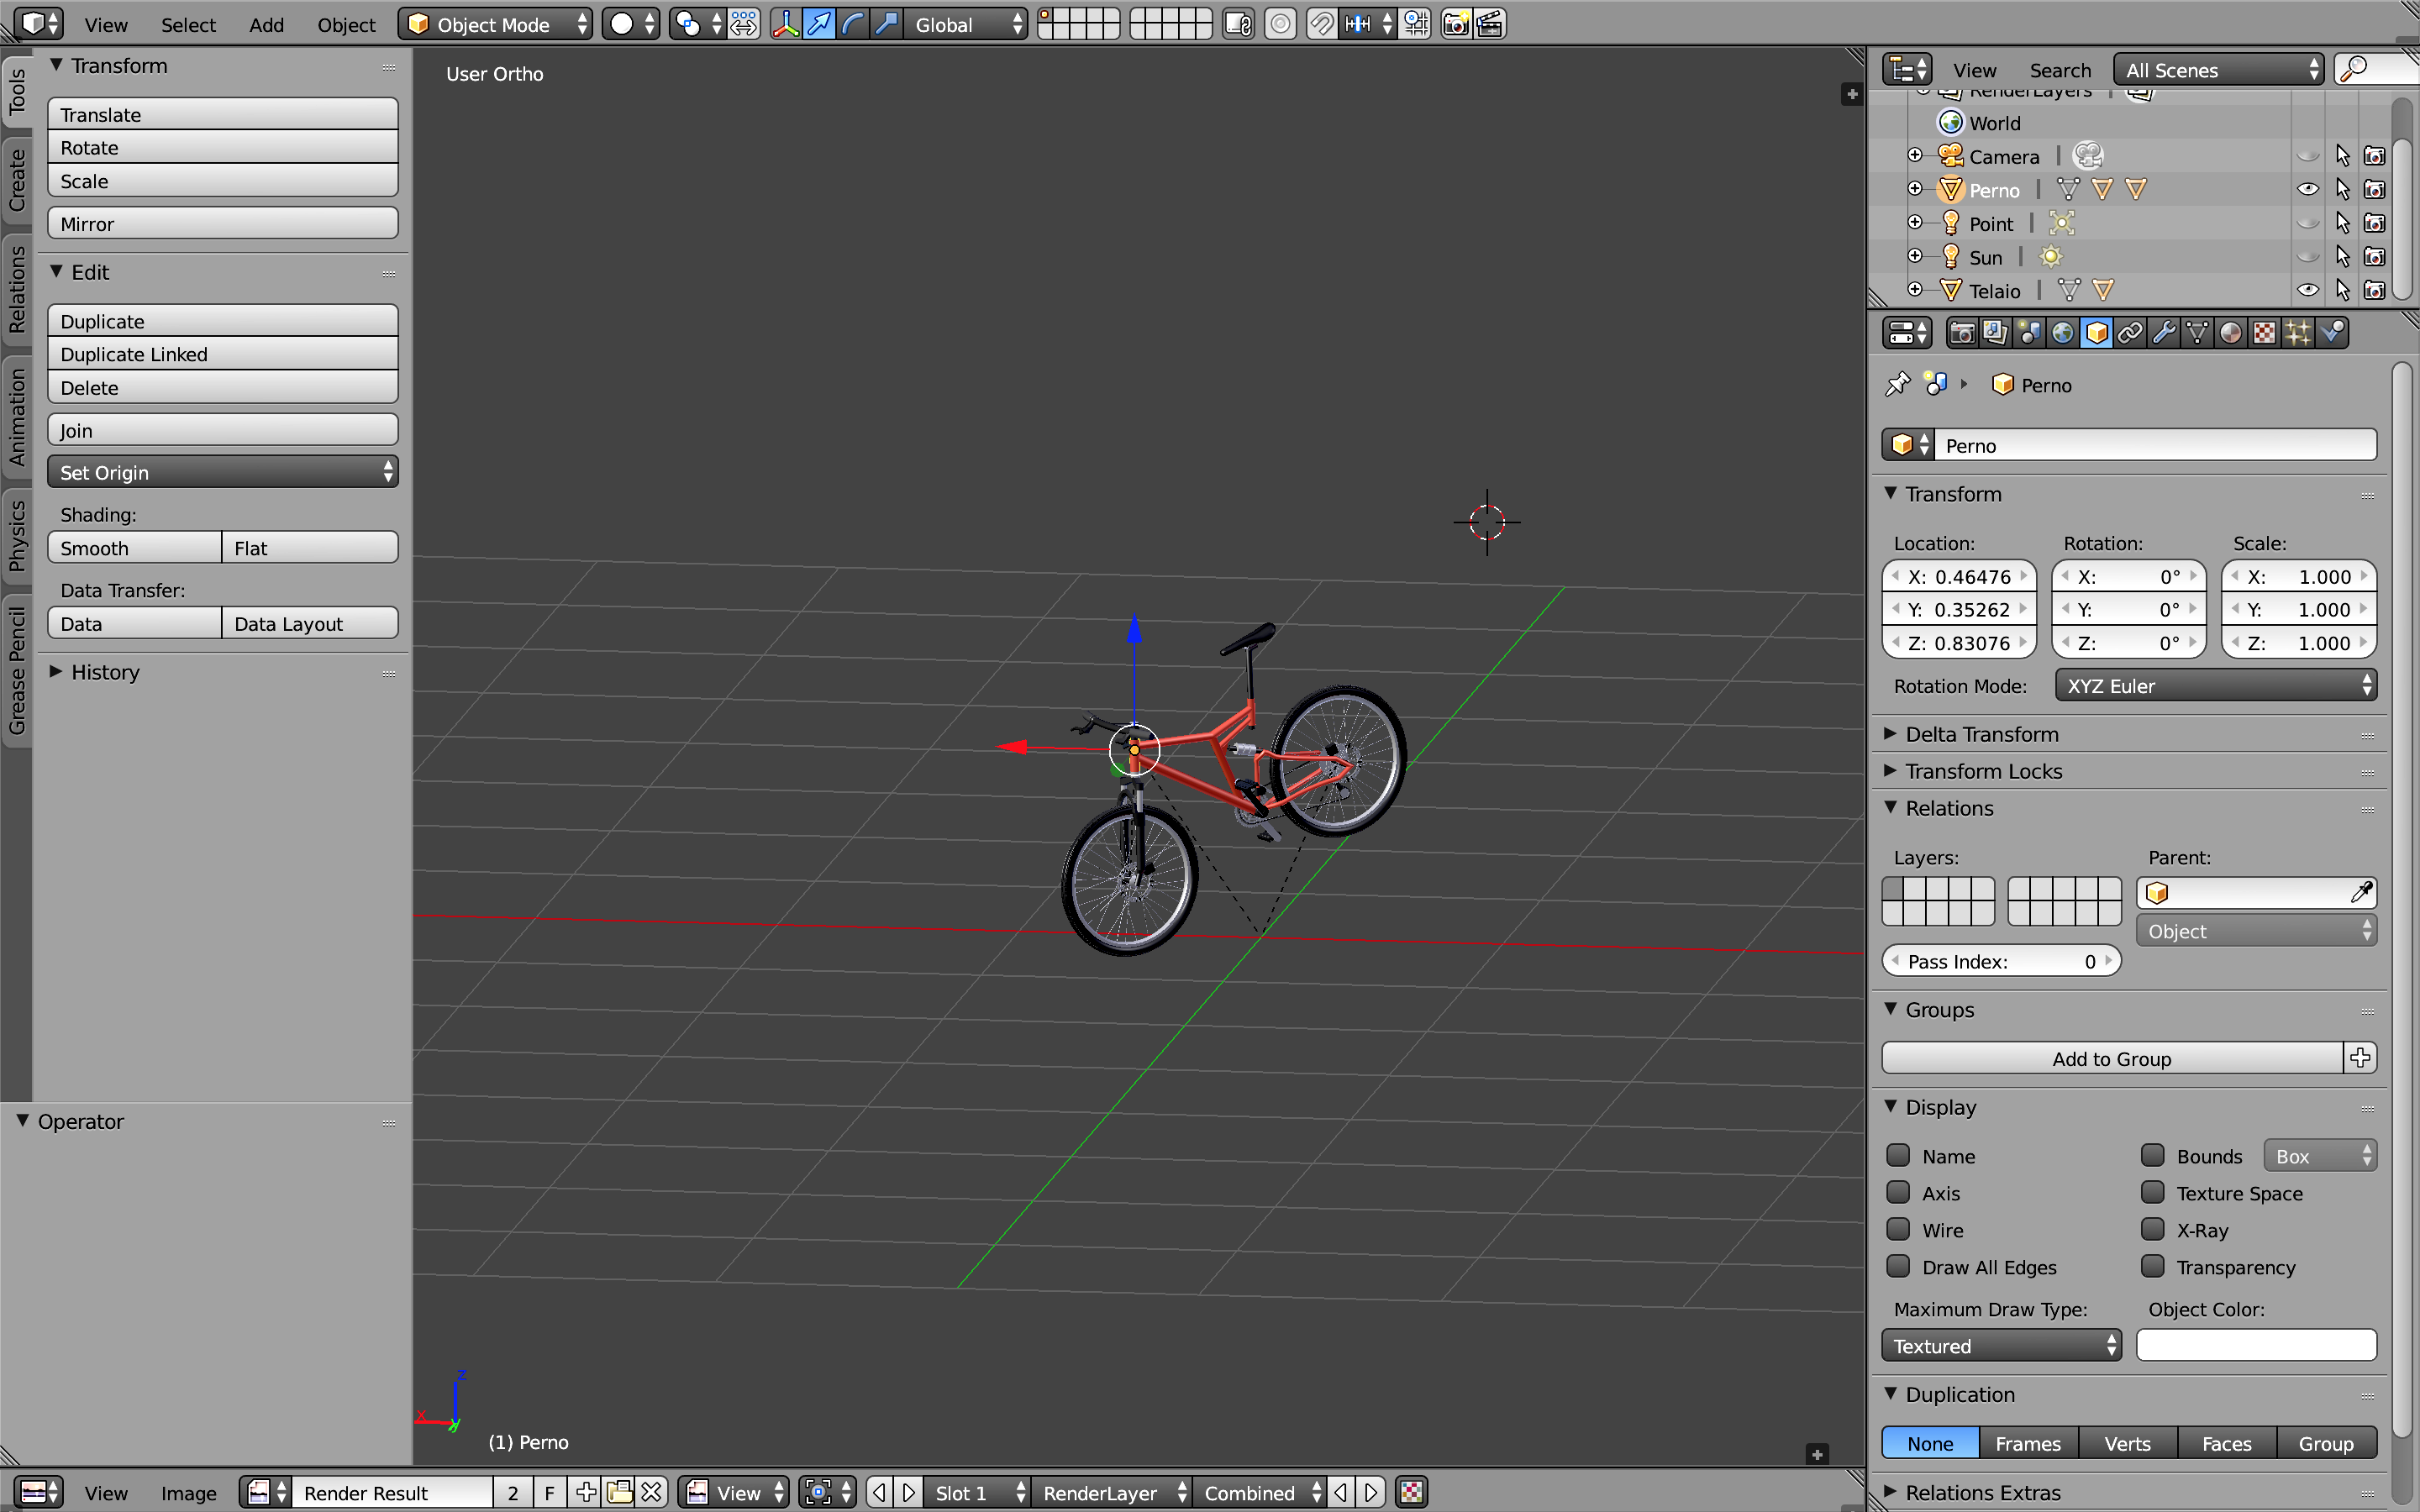
\includegraphics[height=8cm]{schermoblender.png}
  \caption{Interfaccia Principale di Blender}
\end{figure}

\noindent L'\textit{Object Mode} è la modalità che permette di visualizzare le mesh\footnote{Una mesh poligonale, anche detta maglia poligonale, è una collezione di vertici, spigoli e facce che definiscono la forma di un oggetto poliedrico nella computer grafica 3D e nella modellazione solida.} dell'oggetto, mentre l'\textit{Edit Mode} permette di modificarlo. Vi sono altre modalità che non sono state utilizzate, ma risultano utili per una modellazione più dettagliata. Per dotare il modello di texture o di materiali, ovvero l'applicazione di colori, trasparenza, lucentezza o altro, Blender implementa diverse finestre come la \textit{UV/Image Editor} nella quale è possibile scegliere la texture da applicare all'oggetto. Blender è stato utilizzato per creare la mesh della bicicletta virtuale da manovrare attraverso script collegati ad un motore grafico.
\subsection{Mesh della bicicletta}
%\begin{wrapfigure}{l}{0.5\textwidth} %this figure will be at the left
%    \centering
%    \vspace{-0.5cm}
%    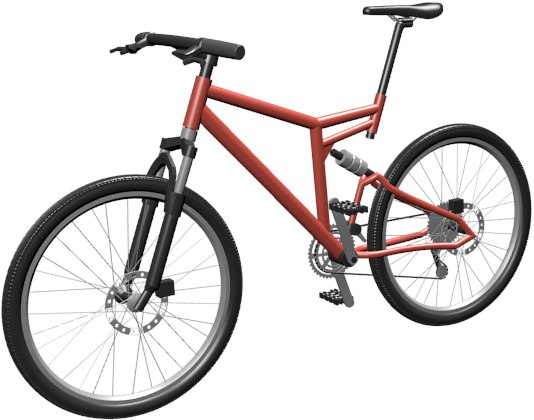
\includegraphics[height=5cm]{meshbici}
%\end{wrapfigure}
 \begin{figure}[htb]
    \centering
    %\vspace{-0.7cm}GameObject
    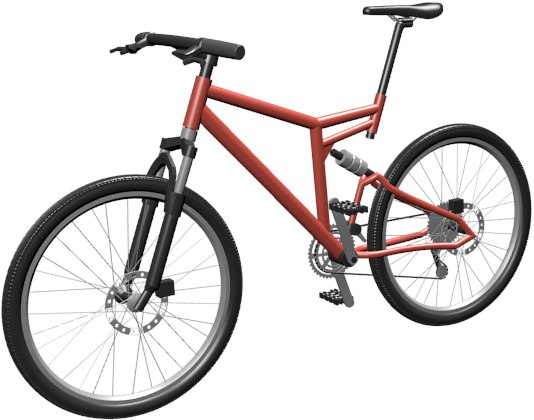
\includegraphics[height=8cm]{meshbici}
%    \caption{\label{fig:meshbici}}
    %\vspace{-0.3cm}
\end{figure}
\noindent La mesh proviene dal sito TurboSquid. È stata scaricata gratuitamente con estensione FBX\footnote{FBX è un formato di file di Autodesk che viene supportato dai più comuni software di grafica 3D in quanto è in grado di immagazzinare non solo geometrie, ma anche dati di texture e di animazioni.} ed è stata adattata per l'utilizzo necessario ai fini del progetto. È stata ridotta in scala ed è stata centrata alle coordinate (0,0,0). La mesh scaricata era già suddivisa in tutti i componenti di una bicicletta classica. Le uniche parti che devono essere dissociate ai fini della tesi sono il manubrio e il telaio. Sono state quindi assemblate tutte le mesh che compongono il telaio e tutte quelle che compongono il manubrio. Blender permette di associare un centro ad ogni mesh con la funzione \texttt{Set Origin > Origin to Geometry}. Questa permette di fornire, a tempo di esecuzione, una rotazione attorno al centro così definito. Sono state quindi lasciate libere le ruote e sono state centrate nel loro origine, in modo da poter dare una rotazione attorno al proprio asse.
\noindent La mesh della bicicletta è stata quindi suddivisa come segue:
\begin{itemize}
  \item \textbf{Telaio}: comprende tutto il telaio della bicicletta escluso il manubrio e le ruote.
	\begin{itemize}
  \item \textbf{Ruota posteriore}: è stata separata per darle possibilità di ruotare sul suo asse.
 \end{itemize}
  \item \textbf{Perno}: consiste nell'unione tra ruota e manubrio. Questo oggetto permette di ruotare tutto il manubrio mantenendo però un asse di rotazione inclinato. Comprende:
 \begin{itemize}
 \item \textbf{Manubrio}: contiene il manubrio stesso, la forcella e l'asse di sterzo.
 \item \textbf{Ruota anteriore}: è stata separata per darle la possibilità di ruotare sul suo asse.
 \end{itemize}
\end{itemize}

\begin{wrapfigure}{r}{0.35\textwidth} %this figure will be at the right
    \centering
    \vspace{-1.3cm}
    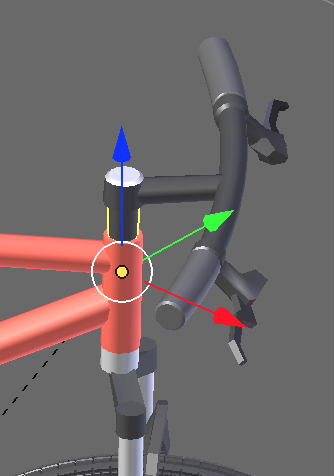
\includegraphics[height=5.5cm]{assebici}
    \caption{L'asse del canotto della bicicletta}
    \vspace{-1.3cm}
\end{wrapfigure}
\noindent Il telaio è stato separato dal manubrio solo nell'asse di sterzo, ma è stato mantenuto il canotto di sterzo, in modo da poter ruotare il manubrio attorno all'asse passante per il centro del canotto. La mesh così ottenuta è stata esportata ed è stata importata in Unity come oggetto da manovrare tramite script.\\
\subsection{Mesh dell'ambientazione}
\label{ambientazione}
\noindent Sono state utilizzate due diverse ambientazioni. La prima delle due è stata fornita dal Cineca: si tratta di un modello 3D dei portici di San Luca (Bologna) ottenuto tramite rilevazione laser. Il modello riporta fedelmente tutti i dettagli spaziali dei portici, ma non riportano la texture. La seconda ambientazione è stata scaricata gratuitamente dallo store di Unity. Per il progetto che è stato creato, l'ambientazione non ha alcuna rilevanza: è possibile asportare la bicicletta e posizionarla in un qualsiasi altro mondo virtuale, purché sia adatto al movimento di una bicicletta al suo interno. L'ambientazione può essere munita di luce principale sia su blender che sul motore grafico. L'importante è non sovrapporre troppe luci per non rischiare la sovra esposizione. In figura \ref{ambientazione} possiamo notare un esempio delle due ambientazioni.
\vspace{-0.5cm}
\begin{figure}[hbp]%
    \centering
    \subfloat[I portici di San Luca]{{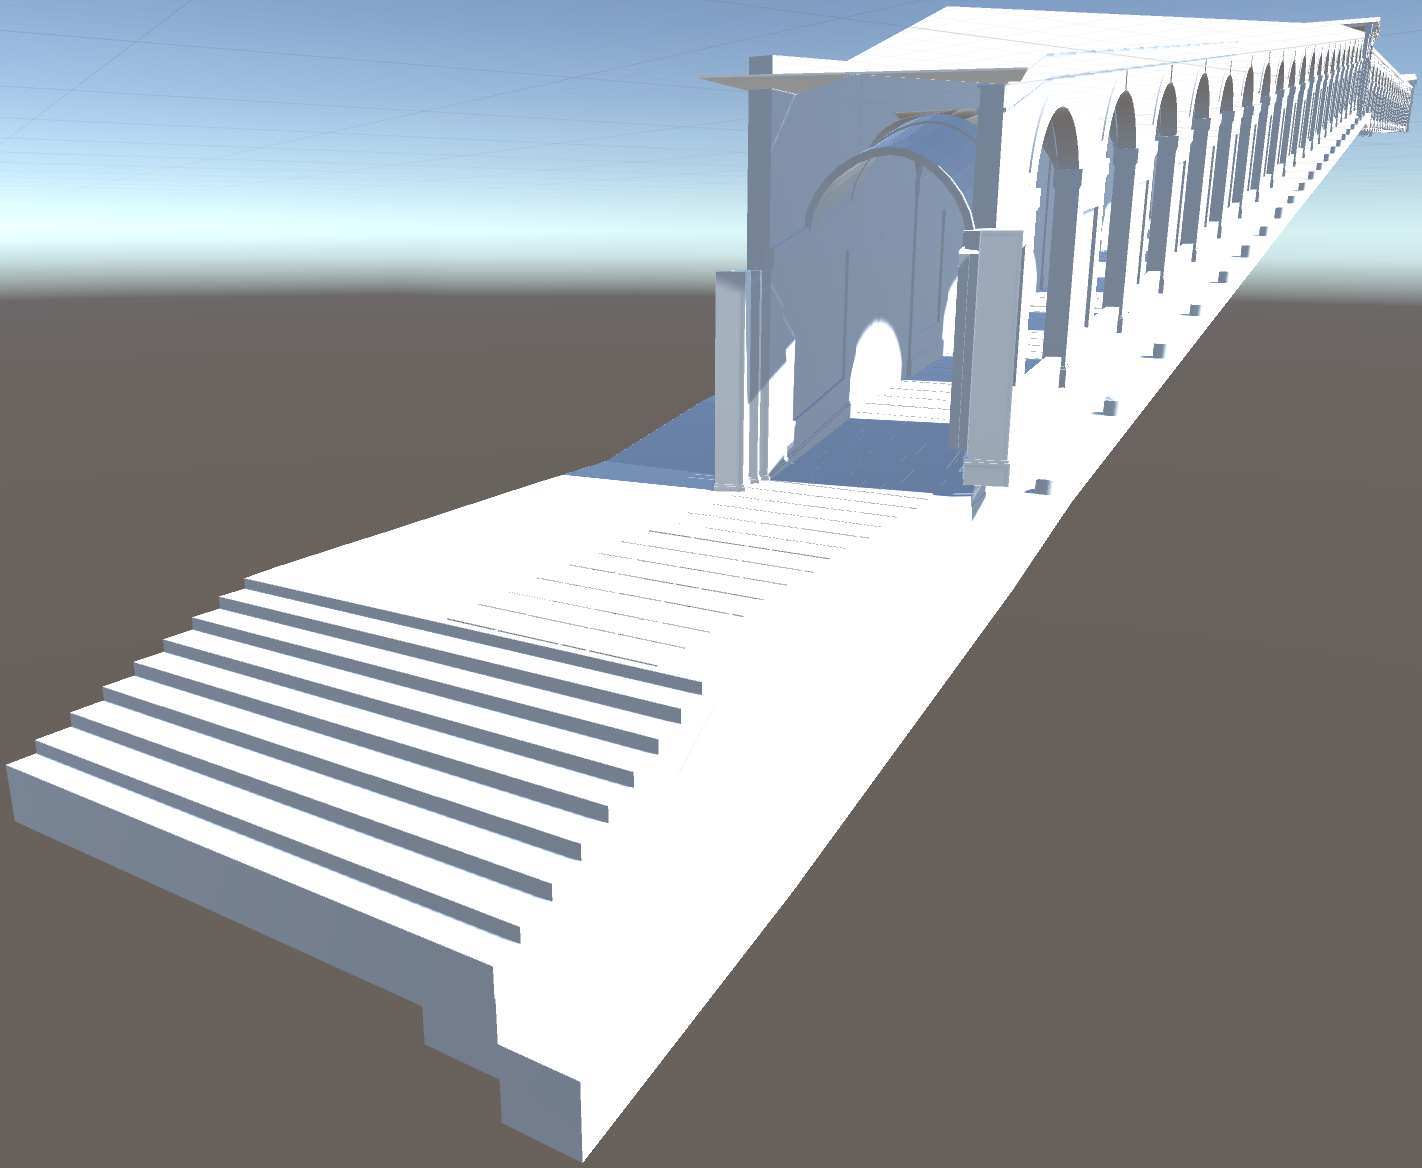
\includegraphics[height=5.5cm]{portici} }}%
    \subfloat[Il tracciato di gara]{{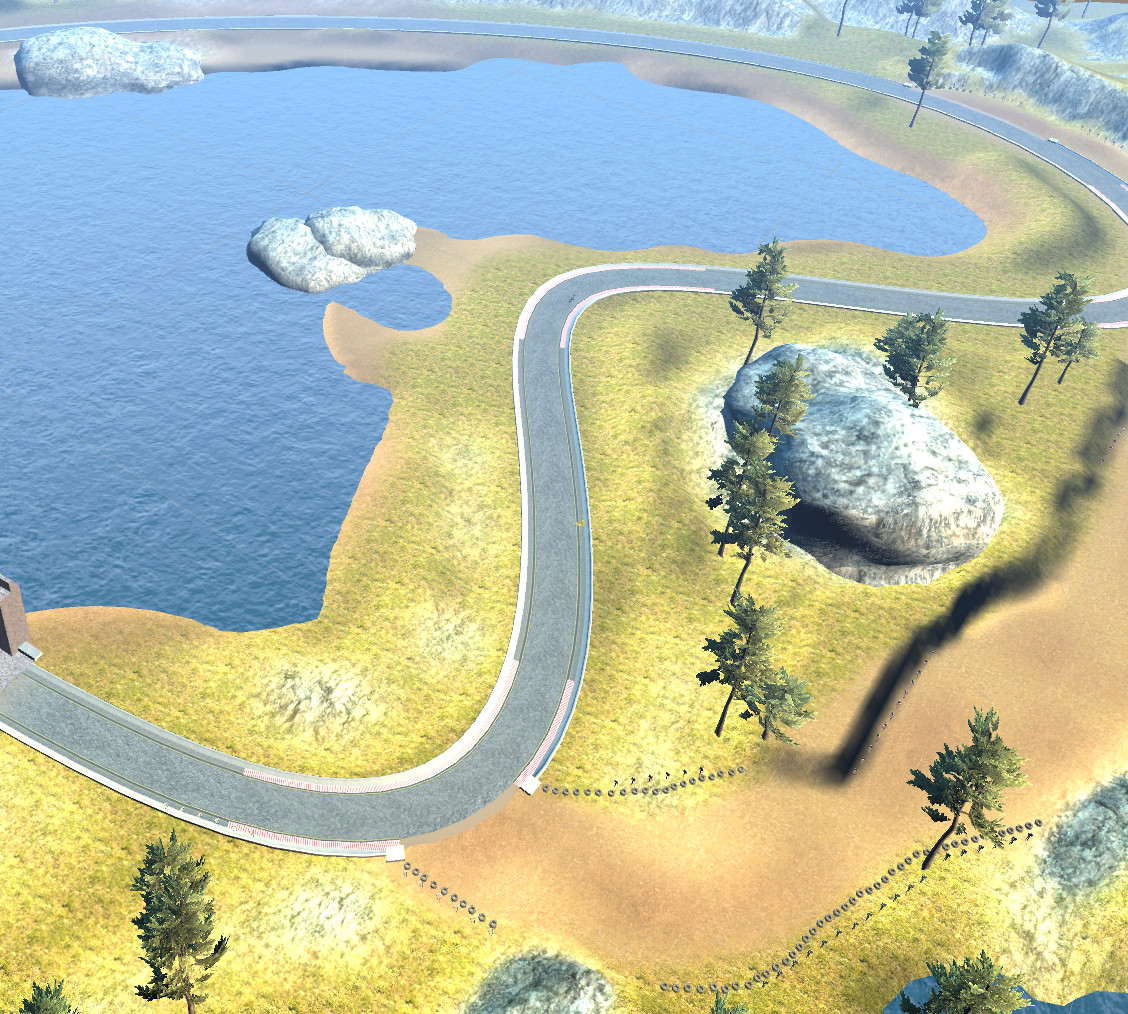
\includegraphics[height=5.5cm]{tracciato} }}%
    \caption{Le due ambientazioni del progetto}%
    \label{ambientazione}
\end{figure}
\vspace{-0.5cm}

\section{Unity}
\noindent 
\begin{wrapfigure}{r}{0.2\textwidth} %this figure will be at the right
    \centering
    \vspace{-1.3cm}
    
\includegraphics[height=3cm]{unityicon}
    \vspace{-1.3cm}
\end{wrapfigure}
Unity è un motore grafico integrato multipiattaforma per la creazione di videogiochi o altri contenuti interattivi 3D, quali visualizzazioni architettoniche o animazioni 3D in tempo reale. Unity permette di modellare l'ambientazione 3D e il modello della bicicletta virtuale attraverso script. Permette inoltre di integrare il visore per la Realtà Virtuale ed è per questo che la scelta è ricaduta su questo motore grafico: per via della facile integrazione dei visori quali OSVR e Oculus Rift.


\subsection{Schermata Principale}
\begin{figure}[htb]
    \centering
    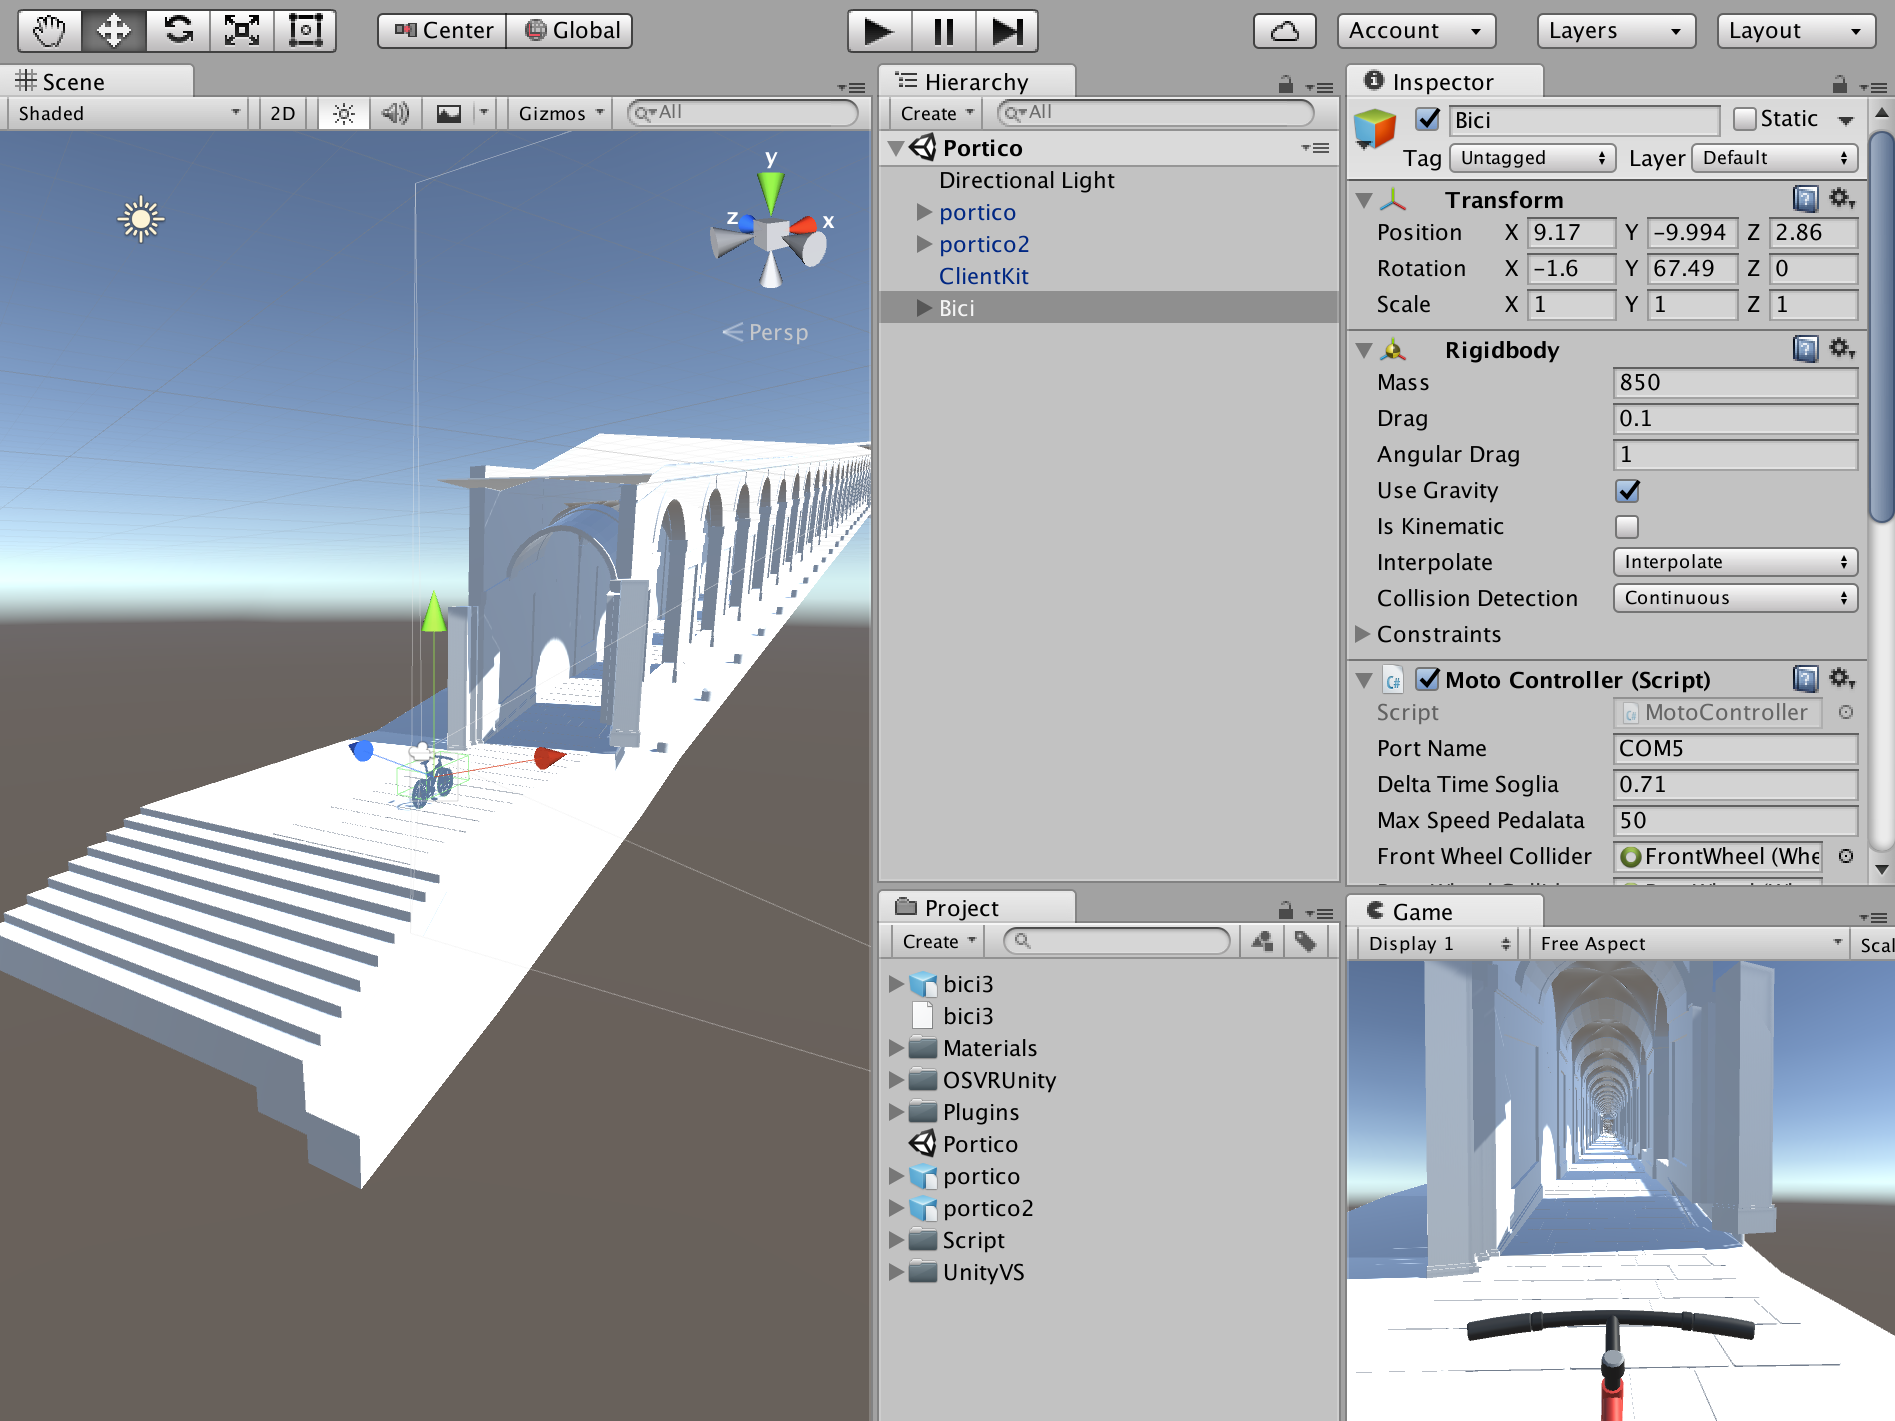
\includegraphics[width=\textwidth]{screenunity}
    \caption{La schermata principale di Unity\label{fig:screenunity}}
    \vspace{-0.3cm}
\end{figure}

\noindent La schermata principale di figura \nameref{fig:screenunity} si compone di 5 riquadri suddivisi in:
\begin{itemize}
  \item \textbf{Scene}: dove viene mostrata l'architettura dell'ambientazione e degli oggetti. All'interno di quest'area si ha la possibilità di modificare gli oggetti, scalarli, muoverli e/o ruotarli. È inoltre possibile cambiare visualizzazione e vista utilizzando mouse e tastiera.
 \item \textbf{Game}: in questo riquadro è possibile osservare l'inquadratura della telecamera o del visore quando la simulazione è avviata. È inoltre possibile interagire con tastiera per muovere gli oggetti o spostare la visuale.
  \item \textbf{Inspector}: questo pannello permette allo sviluppatore di modificare tutti i valori relativo ad un oggetto selezionato. Permette inoltre di assegnare script che modellino a tempo di esecuzione l'oggetto, come ad esempio modificandone la posizione e/o creando animazioni per muoverlo. 
  \item \textbf{Hierarchy}: in questo punto sono elencati tutti gli oggetti presenti nella scena in ordine di parentela o di directory. Ogni componente può averne al suo interno altre (figlie) e può essere usata per trasferire delle caratteristiche quali la posizione, la rotazione e/o vincolare quest'ultime ai comportamenti del padre. Grazie al pulsante Create si possono aggiungere nuovi elementi alla scena. Ogni elemento aggiunto può essere messo in gerarchia semplicemente trascinandolo su un altro con il mouse, questi possono essere oggetti 2D e 3D, telecamere, luci, ecc.
    \item \textbf{Project}: in questa sezione è possibile rintracciare tutte le cartelle e i file del progetto. Questa sezione può interagire con Hierarchy: è infatti possibile trascinare oggetti prefabbricati (come ad esempio la bicicletta creata in Blender) e posizionarli nella scena.
\end{itemize}
Ogni oggetto che fa parte del progetto è elencato all’interno del riquadro Project ed ogni oggetto che fa parte della scena si può trovare all’interno di Hierarchy. Gli oggetti all’interno di Hierarchy vengono chiamati GameObject e ognuno di questi può essere salvato come componente Prefab, con tutti i suoi figli, e riutilizzato in tutte le scene come oggetto identicamente uguale al GameObject che lo ha originato. Questa funzione risulta utile nel caso servano istanze multiple dello stesso GameObject all’interno di una o più scene. Quando viene modificato il GameObject originario, le variazioni si propagano a tutte le sue istanze nel programma. Selezionando un GameObject da Hierarchy o anche dalla sezione Project la finestra Inspector si adatta alla caratteristiche in esso contenute. Ogni GameObject possiede al suo interno dei Component che ne definiscono caratteristiche e comportamento.

\subsection{Scenario Principale}
Durante la progettazione sono stati eseguiti due distinti test su due scenari diversi. Il primo test è stato eseguito nel modello dei portici di San Luca ed è servito per testare il comportamento della bicicletta, in relazione alla fisica dell'attrito e dell'inerzia. Il motivo di questa scelta è dovuto alla pendenza dei portici, che portano la bicicletta a discendere per la gravità. Il secondo test è invece stato eseguito nel modello di un percorso di gara, per verificare l'efficenza della pedalata, la velocità e la pendenza della bicicletta durante una sterzata. Tutte le calibrazioni riguardanti la fisica si tratteranno nella sezione \textit{\nameref{sperimentazione}}. In questa sezione si descriverà lo scenario creato inizialmente per testare gli script che modellano il movimento della bicicletta a tempo di esecuzione.
 \begin{figure}[htb]
    \centering
    %\vspace{-0.7cm}
    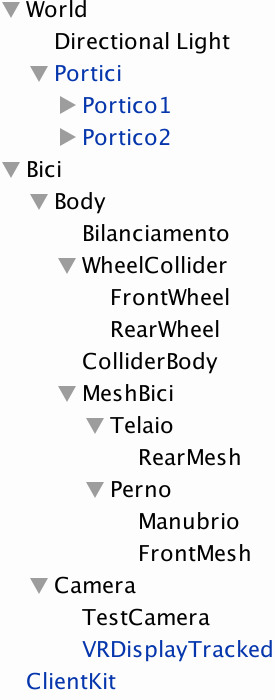
\includegraphics[height=8cm]{hierarchy}
    \caption{La gerarchia di GameObject nello scenario\label{fig:hierarchy}}
    %\vspace{-0.3cm}
\end{figure}
\noindent La gerarchia di GameObject nello scenario è la seguente.
\begin{itemize}
  \item \textbf{World}: Questo oggetto contiene tutti gli elementi del mondo virtuale. Contiene una luce direzionale e può contenere sia il modello dei portici, sia il modello del percorso di gara. Il modello dei portici di San Luca è stato fornito diviso in 2 parti, perciò questi sono stati riuniti in un unico oggetto padre che contiene i due sottogruppi di mesh. Il modello del percorso di gara è stato scaricato da internet come prefabbricato.
  \item \textbf{Bici}: l'oggetto padre contenente altri due oggetti:
		\begin{itemize}
  			\item \textbf{Body}: oggetto contenente le mesh e le meccaniche della bicicletta; i figli saranno vincolati a muoversi in concomitanza dei cambiamenti del suo Component Transform. Il body è un RigidBody: componente utilizzato per rappresentare la fisica dei GameObject composto da diversi dati. Tra i principali ritroviamo la massa assegnata, l’utilizzo o meno della gravità sul dato GameObject e le limitazioni di traslazione e rotazione. Al suo interno vi sono:
					\begin{itemize}
			  			\item \textit{Bilanciamento}: un oggetto che rappresenta il centro di massa della bicicletta su cui si concentrerà il peso. Questo è utile quando la bicicletta effettua salti, infatti le permette di non rovesciarsi.
			  			\item \textit{WheelCollider}: oggetto che contiene i collider delle due ruote, ovvero i GameObject che permettono di collidere con altri oggetti dello stesso tipo. Questi non permettono soloamente alla bicicletta di rimanere ancorata ad un terreno e di non attraversarlo, ma ruotando, forniscono anche il movimento.
						\item \textit{ColliderBody}: è stato aggiunto come involucro esterno per la collisione con l’ambiente circostante. Lo scopo è quello di rendere più realistico l'impatto, al momento della collisione della bici con i muri, evitando che le mesh visibili entrino per metà negli oggetti con cui si scontrano, prima di fermarsi.
						\item \textit{MeshBici}: contiene tutte le mesh della bicicletta. È suddiviso in due elementi: \textit{Telaio} e \textit{Perno}. Il telaio contiene la mesh della ruota posteriore e di tutto il telaio escluso il manubrio. Il perno è l'oggetto che contiene il manubrio e la mesh della ruota anteriore. È una mesh separata poiché permette in base a dove si deciderà di voltare, di avere un feedback visivo della scelta effettuata.
					\end{itemize}
			\item \textbf{Camera}: oggetto contenente due oggetti camera.   		\begin{itemize}
  						\item \textit{TestCamera}: camera solitamente disattivata. Utilizzata solamente in test senza il visore.
			  			\item \textit{VRDisplayTracked}: il Prefab\footnote{Oggetto prefabbricato di Unity, pronto per essere importato} del visore che sostituisce un normale oggetto camera. Questo oggetto camera permettere di essere ruotata tramite i movimenti del visore.
					\end{itemize}
		\end{itemize}
	\item \textbf{ClientKit}: Prefab di OSVR che si occupa del collegamento con il server e i relativi controlli tra il visore e il calcolatore.

\end{itemize}


\noindent Il funzionamento del WheelCollider è vincolato ad avere almeno un RigidBody come padre, questo sarà il componente sul quale verranno applicate tutte le forze di spostamento date dalla torsione delle ruote. Il RigidBody è stato impostato opportunamente ed è stato aggiunto uno script al GameObject per ricevere i segnali di input, per applicare forze alle ruote e per risolvere i limiti della fisica di Unity3D connessi ad esse. Lo script è stato generato vuoto aggiungendo il \textit{Component New Script} attraverso il tasto \textit{Add Component} nel riquadro \textit{Inspector}. Questo script è il \textit{MotoController} e fa uso di una classe \textit{DataReceiver} che si occupa di ricevere i dati dalla cyclette.

\newpage
\section{DataReceiver script}
Questa sezione descrive il comportamento dello script DataReceiver. Questo è stato fornito in versione completa nell'appendice \nameref{receiver} a pagina \pageref{receiver}. Lo script \textit{DataReceiver} si occupa di leggere i dati inviati dal microcontrollore della cyclette alla porta COM del computer e di interpretarli. È costituito da un costruttore, due funzioni private e due pubbliche:
\begin{itemize}
  \item \textbf{Costruttore}: permette di inizializzare la classe \textit{DataReceiver} per utilizzarla nella classe \textit{MotoController}. Esso inizializza il nome della porta COM utilizzata dal ricevitore Bluetooth e imposta la variabile pubblica \textit{go} a true. Questa variabile accessibile anche dal \textit{MotoController}, determina se il thread associato allo script deve continuare o no la lettura dalla porta.
\begin{lstlisting}{Costruttore}
public bool go;
private SerialPort serial;
private string _com;

public DataReceiver(string ComName) 
{
	go = true;
	_com = ComName;
}
\end{lstlisting}

  \item \textbf{Funzioni private}: queste funzioni si occupano di gestire la porta seriale COM.
\begin{itemize}
   \item \textbf{openPort}: si occupa di aprire la porta. Inizializza un oggetto \textit{SerialPort} a 9600bit/s di velocità, senza bit di parità, 8bit di dato e con un solo bit di stop. A questo oggetto assegna un buffer di lettura di dimensione 4096bit e abilita il Data Terminal Ready, un bit di controllo che può indicare l'intenzione di comunicare da parte del dispositivo. È stato necessario configurare un \textit{timeout} di 2 secondi alla lettura della porta. Questo per evitare che, alla chiusura dell'applicazione, il thread associato alla lettura rimanesse in attesa di un dato e bloccasse tutto il sistema. Infine viene fatta l'apertura della porta. La parte principale del metodo è riportata in seguito.
\begin{lstlisting}
serial = new SerialPort(_com, 9600, Parity.None, 8, StopBits.One);
serial.ReadBufferSize = 4096;
serial.DtrEnable = true;
serial.ReadTimeout = 2000; 		
serial.Open();
\end{lstlisting}

   \item \textbf{closePort}: si occupa della chiusura della porta seriale COM. Non fa altro che tentare di eseguire \texttt{serial.Close();} catturando eventuali eccezioni.
   \item \textbf{getData}: riceve e restituisce i dati della seriale sotto forma di stringa solo nel caso in cui lo script sia abilitato alla lettura, ovvero la variabile \textit{go} sia impostata a \textit{true}. Il codice eseguito è il seguente:
\begin{lstlisting}
String tmp = "";
if (serial.IsOpen && go)
	tmp = serial.ReadLine();
return tmp;
\end{lstlisting}
\end{itemize}%funzioni private

  \item \textbf{Funzioni pubbliche}: si basano sullo stato della variabile booleana \textit{go}. Se è \textit{true}, allora il processo abilitato alla lettura deve procedere, altrimenti deve chiudere la porta seriale e terminare la sua esecuzione. Queste funzioni sono richiamate ricorsivamente in \textit{MotoController} e utilizzano le funzioni private sopra definite.
\begin{itemize}
   \item \textbf{start}: apre la porta con \texttt{openPort} ed esegue \texttt{getData} iterativamente con un ciclo \textit{while}, finché \textit{go} è \textit{true}. Ogni volta che legge il dato, lo immagazzina in una stringa e lo suddivide in due valori: \textit{sterzo} e \textit{velocità} che poi invia ad Unity tramite l'evento \textit{PedalataTrovata}. Nel caso in cui \textit{go} sia \textit{false}, il processo esce dal ciclo ed esegue la chiusura della porta tramite \texttt{closePort}. La parsificazione eseguita all'interno del ciclo è descritta nel modo seguente(rimando alla sottosezione \textit{\nameref{stringa}} di pagina \pageref{stringa} per la composizione della stringa inviata dal microcontrollore):
\begin{lstlisting}
//gestione sterzo
tmp = "";
if (data[0] != '0')
tmp += data[0];
tmp += data[1];
sterzo = int.Parse(tmp);

//gestione velocita'
tmp = "";
if (data[3] != '0')
tmp += data[3];
tmp += data.Substring(4);
speed = float.Parse(tmp);
if (speed > 0 && data[2] == '-')
speed *= -1;

//Invio dati a unity
PedalataTrovata(sterzo, speed);
\end{lstlisting}

\item \textbf{stop}: semplicemente imposta la variabile \textit{go} a \textit{false}: \texttt{go = false;}. Questo obbliga il processo a terminare l'esecuzione uscendo dal ciclo \textit{while} sopra descritto.
\end{itemize}%funzioni pubbliche
\end{itemize}%funzioni
\newpage

\section{Motocontroller script}
Il \texttt{MotoController} è lo script direttamente applicato al GameObject \textit{Bici} e lo modella in relazione ai dati ricevuti dalla cyclette.
Al suo interno sono state inserite delle variabili pubbliche affinché siano accessibili direttamente dall’\textit{Inspector} in modo tale da poter aggiungere i vari GameObject di cui si necessita senza doverli cercare da codice. Unity3D al momento del lancio dell’applicazione si preoccupa di collegare alle variabili gli oggetti che sono stati registrati attraverso la schermata di progettazione, come si può vedere dall’immagine seguente.
 \begin{figure}[htb]
    \centering
    %\vspace{-0.7cm}
    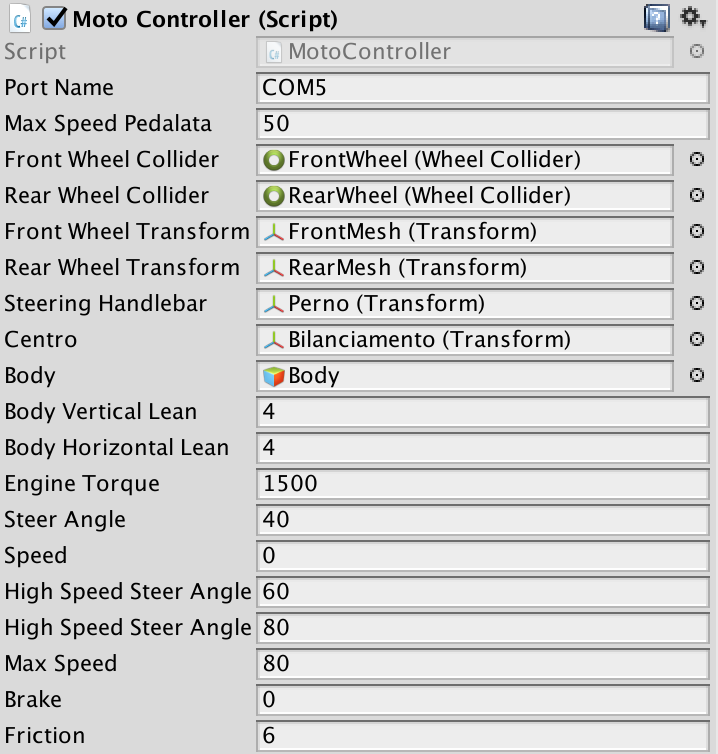
\includegraphics[height=8cm]{variabiliinspector}
    \caption{Le variabili impostabili direttamente dall'inspector di Unity\label{fig:variabiliinspector}}
    %\vspace{-0.3cm}
\end{figure}

\noindent Lo script è una classe che estende \texttt{MonoBehaviour}, una classe di default di Unity per modellare il comportamento di un GameObject. I campi dello Script MotoController.cs visibili nella schermata Inspector di Unity3D per il testing, sono:
\begin{itemize}
  \item Front/RearWheelCollider, rispettivamente i WheelCollider della ruota anteriore e posteriore.
  \item Front/RearWheelTransform, classi Transform collegate ai GameObject delle mesh delle ruote per i movimenti nello spazio e la rotazione della ruota anterore, in modo da dare l’effetto di movimento.
  \item SteeringHandleBar, Transform collegato alla mesh del manubrio per la rotazione nelle curve.
  \item Centro, componente per il calcolo del centro di massa.
  \item Body, GameObject che racchiude in sè tutti i componenti mobili appartenenti alla bici i quali dovranno inclinarsi durante una curva.
  \item Body Vertical Lean, vincolo sull’inclinazione verticale.
  \item Body Horizonatal Lean, vincolo per l’inclinazione orizzontale.
  \item Engine Torque, forza di torsione della ruota.
  \item Steer Angle, vincolo sull’angolo di sterzata massima.
  \item High Speed Steer Angle, angolo di sterzata ad alta velocità.
  \item High Speed Steer Angle At Speed, angolo di sterzata per velocità.
  \item Max Speed, limitatore di velocità.
  \item Brake, forza di frenata.
  \item Friction, forza di attrito.
\end{itemize}

\noindent Tutte le variabili giocano un ruolo fondamentale per il calcolo del movimento e la visualizzazione conseguente. All’interno delle funzioni che si mostreranno sotto, possiamo notarne il comportamento. Si è tuttavia omesso gran parte del codice per rendere più semplice la lettura di questa sezione. Si rimanda quindi all'appendice \nameref{controller} a pagina \pageref{controller}.
\begin{itemize}
	
	\item La funzione \texttt{Start} è la prima ad essere invocata subito dopo il popolamento delle variabili pubbliche, grazie ad essa è possibile:
  	\begin{itemize}
  		\item Salvare il collegamento al \textit{RigidBody}, in questo caso il GameObject, che contiene tutti gli altri, nella variabile \textit{rigid}.
  		\item Imporre vincoli sul movimento della rotazione dell’asse z, impedendo la rotazione.
  		\item Fissare il centro di massa calcolandolo partendo da quello standard e dal GameObject \textit{Bilanciamento}
  		\item Stabilire un limite alla velocità angolare
  		\item Salvare la preferenza per l’angolo di sterzata
  		\item Inizializzare il Receiver e impostare l'evento PedalataTrovata
  		\item Creare un thread separato che esegua il codice del Receiver.
	\end{itemize}
	
	\item \texttt{FixedUpdate} area che va utilizzata per la modifica dei GameObject che possiedono il Component RigidBody. All’interno invochiamo tre funzioni per il controllo degli input, quali l’attivazione del movimento delle ruote, l’eventuale arresto o retromarcia. Queste funzioni sono state definite sotto e sono:
		\begin{itemize}
			\item Inputs
			\item Engine
			\item Braking
		\end{itemize}
		
	\item \texttt{Update} viene richiamato in concomitanza con \texttt{Fixed\-Update} ed è indispensabile in quanto è l’unico metodo disponibile per l’aggiornamento dalla grafica. Al suo interno troviamo altre due funzioni utili per aggiornare i movimenti delle mesh su schermo e per controllare l’angolo del nostro assetto verticale:		\begin{itemize}
			\item WheelAlign
			\item Lean
		\end{itemize}
	
	\item \texttt{Inputs} controlla lo stato degli input e modifica le variabili che serviranno per calcolare il movimento che dovrà essere effettuato, nel dettaglio:
		\begin{itemize}
			\item Salva la velocità corrente convertita.
			\item Riporta i dati delle rotazioni imponendo quella sull’asse z a 0.
			\item Imposta la variabile che discrimina il movimento in avanti o all’indietro.
			\item Inserisce il valore della variabile per l’angolo di sterzata
			\item Controlla e imposta la variabile per la retromarcia.
		\end{itemize}
		
	\item \texttt{Engine} mette in moto i WheelCollider e permette quindi alla bicicletta di sostenere un moto accelerato. Il procedimento sarà quello di:
		\begin{itemize}
			\item Calcolare l’angolo di sterzata contenuta nelle variabili precedentemente ottenute grazie agli ingressi e imporle al Collider della ruota anteriore.
			\item Trovare la velocità da inserire. In base al valore che questa assume distinguiamo due comportamenti:
			\begin{itemize}
			  \item Il primo cessa l’accelerazione per il superamento della velocità massima, subendo l’inerzia fino al momento in cui non si torni al di sotto della soglia consentita riaccelerando.
			  \item Il secondo applica la forza di accelerazione il parametro \textit{motorTorque}
			\end{itemize}
			\item Controllare sul reversing: nel caso in cui l’input sia una velocità negativa, si impone questa pari a:
			\begin{itemize}
			  \item 0 per velocità maggiori di quella desiderata
			  \item una velocità di retromarcia ridotta.
			\end{itemize}
		\end{itemize}
		
		\item \texttt{Braking} in caso di frenata deceleriamo la bici fino al punto di invertire la marcia. Le opzioni sono:
		\begin{itemize}
			\item Se la velocità è inferiore da una certa soglia, rilasciando il tasto di input viene applicato un attrito che permetterà alla bici di fermarsi. Esso mantiene il mezzo fermo anche in caso di dislivello.
			\item Se applico un valore negativo di input e non siamo in retromarcia, si avrà una frenata più rapida.
			\item Se non si è in nessuno dei due precedenti casi, la forza di decelerazione viene resa nulla.
		\end{itemize}
		
		\item \texttt{WheelAlign} calcola i movimenti che dovranno eseguire le mesh delle ruote e del manubrio in accordo con l’input e i WheelCollider. Le fasi operative saranno:
		\begin{itemize}
			\item Calcolare il punto di contatto con il terreno.
			\item Controllare, tracciando una linea immaginaria dal centro della ruota, se lungo il percorso si incontra un altro Collider.
			\item Disegnare la mesh nel punto calcolato in base ai controlli effettuati.
			\item Adeguare la rotazione in base alla velocità e al tempo del movimento.
			\item Applicare la torsione alla ruota anteriore in base alla rotazione del FrontWheelCollider.
			\item Compiere i passaggi precedenti anche per la ruota posteriore, ovviamente trascurando la torsione derivante dal manubrio.
			\item Ruotare il manubrio in base all’angolo di sterzata. Siccome il manubrio è inclinato e non perfettamente perpendicolare al piano di appoggio, è stato necessario utilizzare Eulero attraverso i parametri \textit{eulerAngles}. Questo è quanto viene applicato:
			\begin{itemize}
			  \item Si ottiene la differenza di angolo tra la posizione corrente (euler.z) e l'angolo del FrontWheelCollider.
			  \item Si applica la formula \texttt{euler.z = \-(euler.z \-- \-angleDifference) \% 360} per fornire la rotazione sull'asse inclinato
			  \item Si applica il valore ottenuto agli \texttt{eulerAngles} del manubrio.
			\end{itemize}

		\end{itemize}
		
		\item \texttt{Lean} calcola e applica l’inclinazione verticale a fronte di una sterzata. Le operazioni contenute in essa sono:
		\begin{itemize}
			\item Calcolare l’angolo rispetto alla verticale in base ai dati e al tempo.
			\item Salvare i dati del contatto con il terreno del WheelCollider.
			\item Utilizzare i dati del contatto per ottenere l’angolo normalizzato in corrispondenza del terreno. Se quest’ultimo, dovesse essere maggiore, rispetto a quello desiderato, verrà limitato da un lato o dall’altro.
			\item Calcolare l’angolo orizzontale.
			\item Generare gli angoli di rotazione e applicarli al Body.
			\item Ricalcolare il centro di massa per non avere effetti anomali, per esempio di trascinamento orizzontale.
		\end{itemize}
		
		\item \texttt{ReceiverPedalataTrovata} funzione per gestire l'oggetto evento di \textit{DataReceiver} e aggiornare le variabili che immagazzinano i valori di sterzo e velocità di pedalata.
		\item \texttt{OnApplicationQuit} funzione che ridefinisce la chiusura dell'applicazione. Richiama la funzione \textit{stop} di \textit{DataReceiver} e si sospende in attesa della terminazione del thread associato.
		\item \texttt{msgToDebug} funzione utile per debug. Permette di scrivere direttamente nella console di debug, una stringa passata come argomento.
	
\end{itemize}

\noindent Un volta scritto, lo script \texttt{Motocontroller} deve essere associato all'oggetto Bici, come in figura \ref{fig:variabiliinspector}. 

\section{OSVR}
Il visore OSVR deve semplicemente sostituire l'oggetto camera con un suo prefabbricato. Questo prefabbricato è impostato per muoversi in relazione ai movimenti del visore. Per utilizzare i prefabbricati e per poter utilizzare il visore è stato necessario installare il software fornito dal portale sviluppatori su Github. I pacchetti che sono stati utilizzati sono tre: il primo per la configurazione del visore e per il controllo del suo funzionamento, il secondo per l'abilitazione dell'accelerometro e del giroscopio tramite l'utilizzo del server (un processo locale) e il terzo per importare sia i componenti da utilizzare sia le scene di testing all'interno di Unity. Utilizzando il secondo pacchetto contenente il server, un processo locale che utilizza un file .json per la configurazione del visore(e quindi è possibile crearsene di personalizzati), si è abilitato il tracker per il rilevamento della posizione e per lo spostamento dell'accelerometro. Completata la configurazione del visore, è stato possibile integrarlo con Unity. Dei componenti importati e necessari su Unity sono stati adoperati il \textit{ClientKit}, che si occupa del collegamento con il server e i relativi controlli tra il visore e il calcolatore, e il \textit{VRVRDisplayTracked} già dotato della camera, che consente di visualizzare la simulazione, e degli script per il movimento all'interno del mondo.


























%
